\chapter{Background and Related Work}
\label{chapter:background}

This section offers background notes, evaluation criterion, and vocabulary which would be used throughout this thesis.

\section{Motivating Example}
To motivate our work, we use the same example from a previous work~\cite{guo2013variability}, a configurable
command-line tool x264 for encoding video streams into the H.264/MPEG-4 AVC format.
In this example, we consider 16 encoder features of x264, such as encoding with multiple
reference frames and parallel encoding on multiple CPUs. The user can select
different features to encode a video. The encoding time is used to indicate the performance
of x264 in different configurations. A configuration represents a program variant with
a certain selection of features. This example with only 16 features gives rise to 1,152
configurations. Intuitively, 16 binary features should provide $2^{16}$ different configurations,
however, in this work we consider only valid configurations i.e. configurations that are
allowed by the system under investigation.
In practice, often only a limited set of configurations can be measured, either by simulation
or by monitoring in the field. For example, Figure~\ref{fig:chap1_random_sample} lists a sample of 16 randomly selected
configurations and their actual performance measurements. How can we determine
the performance of other configurations based on a small random sample of measured configurations?
\begin{figure}[!htbp]
    \centering
    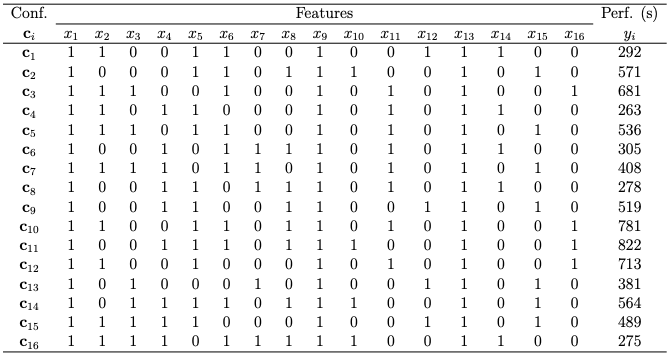
\includegraphics[width=0.8\linewidth]{Figures/table.png}
    \caption[Table with randomly selected configurations]{A sample of 16 randomly-selected configurations of x264 and corresponding
performance measurements (seconds)}
    \label{fig:chap1_random_sample}
\end{figure}
\section{Problem Formulation}
To formulate the above issue, we represent a feature as a binary decision variable x (please note that decision variable could be decimal as well).
If a feature is selected in a configuration, then the corresponding variable is set to 1, and
0 otherwise. Assume that there are $N$ features in total, all features of a program are
represented as a set $X = {x_1, x_2, ..., x_N}$. A configuration is an N-tuple $c$, assigning 1 or 0
to each variable. For example, each configuration of x264 is represented by 16-tuple, e.g.
$c_1$ = ($x_1$ = 1, $x_2$ = 1, $x_3$ = 0, $x_4$ = 0, ..., $x_{16}$ = 1). All valid configurations of a program are
denoted by $C$.
Each configuration $c$ of a program has an actual measured performance value y. Performance values are taken from publicly available dataset deployed with SPLConqueror
tool.
All performance values of  $C$ form set $Y$ . Suppose that we acquire a
random sample of configurations $C_S \in C$ and their actual measured performance values
$Y_S \in Y$ , together forming sample $S$. The problem of variability-aware performance prediction
is to predict the performance of other configurations in $C \in CS$ based on the measured
sample S.
We regard all variables in X as predictors and a configuration\textquotesingle s actual performance
value y as the response. In other words, we predict a quantitative response y based on a
set of categorical predictors X, which is a typical regression problem. \textit{Due to feature
interactions, the above issue is reduced to a non-linear regression problem, where the
response depends non-linearly on one or more predictors.}




\section{Evaluation Metrics: Quality and Cost}
The performance of the methods proposed in this thesis is evaluated the following two metrics:\\
\noindent\textbf{Quality}: Quality of an approach refers to the distance between the solutions returned by the methods proposed and the ground truth (actual measurements). Quality can be calculated as the \textit{rank difference} which is the distance between best solution (also referred to as configuration) found by (proposed) techniques to the actual best solution.

\noindent\textbf{Cost}: Cost of an approach refers to the effort (such as time, money, developer hours) required by an approach to find a good configurations. In this thesis, we use number of measurements (or benchmark runs) as an proxy to the search effort. This is something unique (and surprising that the other work in this area never considered this aspect) about the work presented in this thesis. 

\begin{figure}[!htbp]
    \centering
    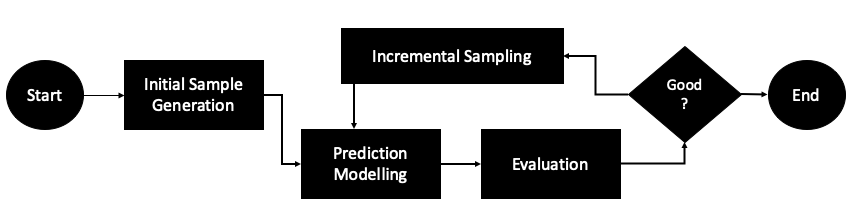
\includegraphics[width=0.8\linewidth]{Chapter-Introduction/Figures/sampling_process.png}
    \caption{General process of performance prediction by sampling}
    \label{fig:chap1_sampling_process}
\end{figure}

\section{Prior Work}
Figure~\ref{fig:chap1_sampling_process} illustrates the general process of performance prediction by sampling. It starts with
an initial sample of measured configurations, which are used to build the prediction model. New configurations are added to iteratively improve the model such that it because reliable. Reliability of the model is measured using MMRE (Mean Magnitude of Relative Error), which is defined as:
\begin{equation}
\mathit{MMRE}=\frac{\mid\mathit{predicted} - \mathit{actual}\mid}{\mathit{actual}}*100
\end{equation}
A good initial sample significantly reduces the iterations of the entire prediction process. State-of-the-art
approaches fix the size of the initial sample to the number of features or potential feature
interactions of a system~\cite{siegmund2012predicting, guo2013variability, sarkar2015cost, jamshidi2016uncertainty}. However, such a strategy might not be the optimal one, as the
number of features (and their interactions) can be high and, at the same time, an acceptable prediction
accuracy might be achieved using a substantially smaller set of measured configurations.

\noindent\textbf{Observation}: Although, the methods proposed by prior work exploited random sampling and CART decision trees (which are both scalable), these methods perform evaluations which are not necessarily useful in finding good configuration. While this approach worked reasonable well with respect to the quality of solutions, it failed to fare well in terms of cost (dual axis). Most of the method proposed in prior work use over 50\% of the configurations (from the configuration space), to build a reliable model. 


\subsection{Related Work}
Many researchers report that modern software systems come with \textcolor{black}{{\em a daunting number of configuration options}}. 
For example, the number of configuration options in Apache (a popular web server) increased from 150 to more than 550 configuration options within 16 years~\cite{xu2015hey}. 
Van Aken et al.~\cite{van2017automatic} also reports a similar trend. They indicate that, in over 15 years, the number of configuration options of {\sc Postgres} and {\sc MySQL} increased by a factor of three and six, respectively.
This is troubling since
Xu et al.~\cite{xu2015hey} report that developers tend to ignore over 80\% of configuration options, which leaves considerable optimization potential untapped and induces major economic cost.\footnote{The size of the configuration space increases exponentially  with the number of configuration options.} 
% \fig{software_systems} offer examples of the kinds of configuration options seen in software systems. 



Finally, another problem  with configurable
systems is the issue of  \textcolor{black}{{\em poorly chosen default configurations}}.
Often, it is assumed that software architects provide useful default configurations of their systems.  This assumption can be very
misleading.   Van Aken et al.~\cite{van2017automatic} report that the default MySQL configurations in 2016 assume that it will be installed on a machine that has  160MB of RAM (which, at that
time, was incorrect by, at least, an order of magnitude). Herodotou et al.~\cite{herodotou2011starfish} show how standard settings for text mining
applications in Hadoop result in worst-case execution times.
In the same vein,  
Jamshidi et al.~\cite{jamshidi2016uncertainty} reports for
 text mining applications on Apache storm, the throughput achieved using the worst configuration is 
{\em 480 times slower} than the throughput achieved by the best configuration.

Yet another  problem
is that 
\textcolor{black}{{\em  exploring benchmark sets for different configurations is very slow}}. 
Wang et al.~\cite{wang2013searching} comments on the problems of evolving a test suite for software if every candidate solution requires a time-consuming execution of the entire system: such test suite generation can take weeks of execution time.
Zuluaga et al.~\cite{zuluaga2013active} report on the cost of analysis for software/hardware co-design: ``synthesis of only one design can take hours or even days''. 

 
 
The challenges of having numerous configuration options are just \textcolor{black}{{\em not limited to software systems}}. The problem to find an optimal set of configuration options is pervasive and faced in numerous other sub-domains of computer science and beyond. In software engineering, software product lines--where the objective is to find a product which (say) reduces cost, defects~\cite{chen2016sampling, henard2015combining}---has been widely studied.  
Interaction testing---how to test configurable systems, when the same test case will behave differently while running under the same set of test cases~\cite{cohen2006testing, qu2007combinatorial, jin2014configurations, medeiros2016comparison}. 
The problem of configuration optimization is present in domains, such as machine learning, cloud computing, and software security.


The area of \textcolor{black}{{\em hyper-parameter optimization}} (a.k.a.  parameter tuning) is very similar to the performance configuration optimization problem studied in this paper. Instead of optimizing the performance of a software system, the hyper-parameter method tries to optimize the performance of a machine learner. Hyper-parameter optimization is an active area of research in various flavors of machine learning. For example, Bergstra and Bengiol~\cite{bergstra2013making} showed how random search could be used for hyper-parameter optimization of high dimensional spaces.
Bergstra et a also showed how to tune computer vision software.
Feurer el al.~\cite{feurer2015initializing} showed how hyper-parameters could affect the performance of a Bayesian optimizer. 
Recently, there has been much interest in 
hyper-parameter optimization applied to the area of software analytics~\cite{fu2016tuning, fufse17, fu2016differential, tantithamthavorn2016automated, agrawal2016wrong}.

Another area of application for performance configuration optimization is \textcolor{black}{{\em cloud computing}}.  
With the advent of big data, long-running analytics jobs are commonplace. Since different analytic jobs have diverse behaviors and resource requirements, choosing the correct virtual machine type
in a  cloud environment has become critical. This problem has received considerable interest, and we argue, this is another useful application of performance configuration optimization --- that is, optimize the performance of a system while minimizing cost~\cite{alipourfard2017cherrypick, venkataraman2016ernest, yadwadkar2017selecting, Zhu:2017:BTP:3127479.3128605, dalibard2017boat}. 


As a sideeffect of the wide-spread adoption of cloud computing, the \textcolor{black}{{\em security}} of the instances or virtual machines (VMs) has become a daunting task. In particular, optimized security settings are not identical in every setup. They depend on characteristics of the setup, on the ways an application is used or on other applications running on the same system. The problem of finding security setting for a VM is similar to performance configuration optimization~\cite{biedermann2014hot, biedermann2014leveraging, drabik2003method, security1, security2}. 
Among numerous other problems which are similar to performance configuration optimization, the problem of how to maximize conversions on landing pages or click-through rates on search-engine result pages~\cite{hill2017efficient, wang2016beyond, zhu2017optimized} has gathered interest.  


